\documentclass{standalone}
\usepackage{pgfplots}
\pgfplotsset{compat=newest}

\begin{document}
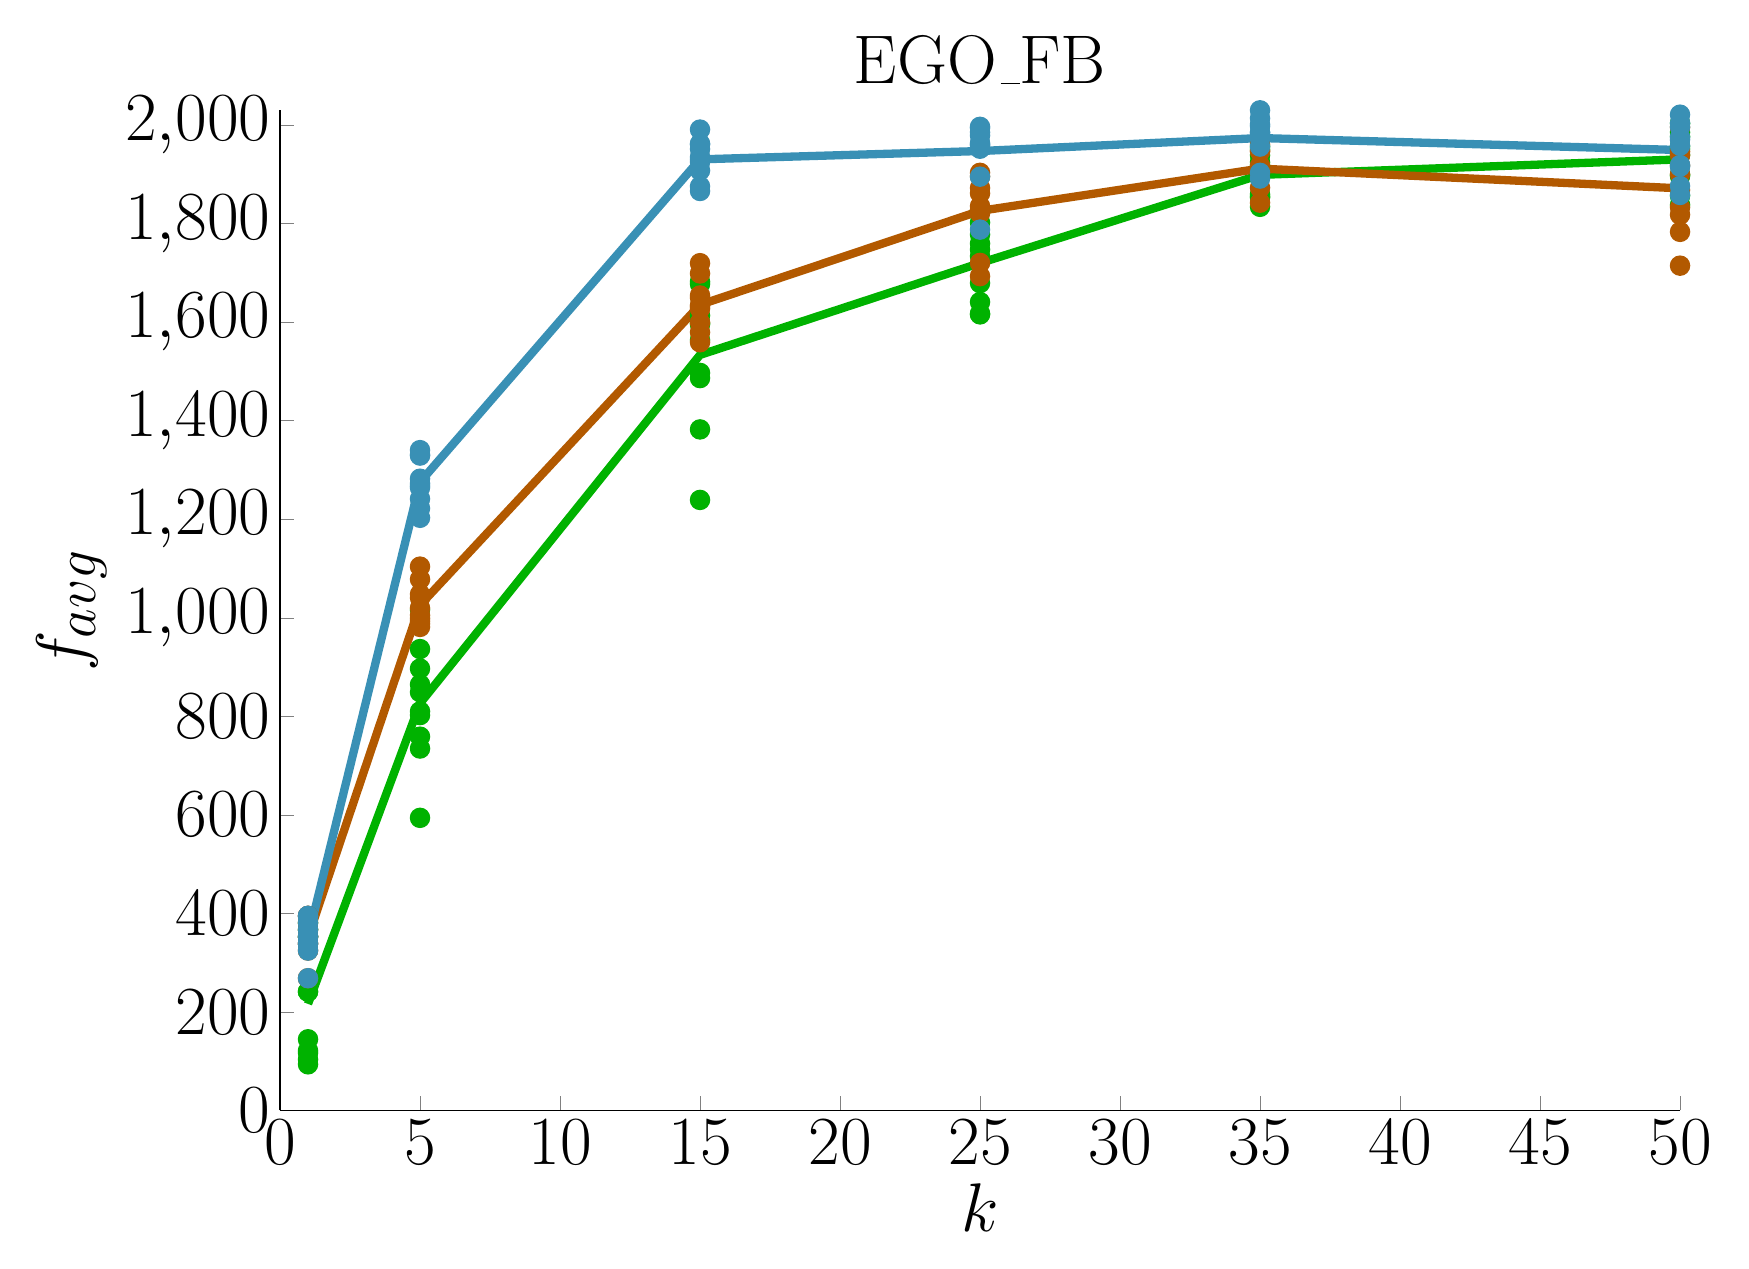
\begin{tikzpicture}

\begin{axis}[%
title style={font=\Huge},
title=EGO\_FB,
tick label style={font=\Huge},
label style={font=\Huge},
legend style={font=\Huge},
view={0}{90},
max space between ticks=50pt,
width=7in,
height=5in,
scale only axis,
xmin=0, xmax=50,
%xtick={0, 20, 40, 60, 80, 100},
xlabel={$k$},
ymin=0, ymax=2030.36,
ylabel={$f_{avg}$},
major tick length=5pt,
axis lines*=left,
legend cell align=left,
clip=false]

\addplot [
only marks,
mark=*,
mark size=3.5pt,
color=green!70!black,
%solid,
%line width=2pt,
]
coordinates{
(1,93.4)(1,103.12)(1,116.44)(1,121.12)(1,144.22)(1,241.0)(1,241.0)(1,352.5)(1,366.56)(1,380.62)(5,593.82)(5,734.56)(5,758.64)(5,802.44)(5,809.88)(5,849.0)(5,864.5)(5,896.84)(5,936.52)(5,1016.12)(15,1239.28)(15,1382.46)(15,1486.68)(15,1497.2)(15,1563.84)(15,1596.14)(15,1598.26)(15,1613.58)(15,1677.7)(15,1682.6)(25,1615.98)(25,1617.5)(25,1641.0)(25,1679.54)(25,1733.9)(25,1747.82)(25,1759.8)(25,1778.16)(25,1802.4)(25,1825.86)(35,1834.42)(35,1853.38)(35,1855.26)(35,1859.94)(35,1899.3)(35,1918.58)(35,1924.72)(35,1939.22)(35,1951.3)(35,1956.26)(50,1838.34)(50,1857.0)(50,1896.9)(50,1899.24)(50,1939.56)(50,1951.94)(50,1957.32)(50,1977.38)(50,1985.68)(50,2003.78)
};

\addplot [
only marks,
mark=*,
mark size=3.5pt,
color=orange!70!black,
%solid,
%line width=2pt,
]
coordinates{
(1,268.14)(1,324.38)(1,338.44)(1,338.44)(1,352.5)(1,352.5)(1,366.56)(1,380.62)(1,394.68)(1,394.68)(5,981.42)(5,987.6)(5,993.18)(5,998.54)(5,1005.04)(5,1019.72)(5,1040.54)(5,1047.88)(5,1078.26)(5,1103.92)(15,1559.36)(15,1579.72)(15,1599.68)(15,1627.26)(15,1631.74)(15,1634.3)(15,1649.66)(15,1654.44)(15,1699.06)(15,1720.0)(25,1693.64)(25,1720.48)(25,1821.26)(25,1827.58)(25,1828.1)(25,1835.74)(25,1862.02)(25,1872.6)(25,1896.48)(25,1903.46)(35,1842.74)(35,1872.96)(35,1901.86)(35,1905.52)(35,1907.54)(35,1915.64)(35,1918.02)(35,1946.54)(35,1947.88)(35,1961.16)(50,1714.94)(50,1783.58)(50,1818.34)(50,1833.44)(50,1868.64)(50,1900.46)(50,1918.22)(50,1939.32)(50,1946.4)(50,1995.96)
};

\addplot [
only marks,
mark=*,
mark size=3.5pt,
color=cyan!70!black,
%solid,
%line width=2pt,
]
coordinates{
(1,268.14)(1,324.38)(1,338.44)(1,338.44)(1,352.5)(1,352.5)(1,366.56)(1,380.62)(1,394.68)(1,394.68)(5,1203.0)(5,1222.06)(5,1241.42)(5,1264.3)(5,1267.84)(5,1272.54)(5,1282.32)(5,1329.34)(5,1331.22)(5,1340.4)(15,1866.56)(15,1875.88)(15,1908.08)(15,1925.16)(15,1930.54)(15,1935.5)(15,1951.6)(15,1960.78)(15,1962.64)(15,1991.24)(25,1788.12)(25,1895.62)(25,1952.38)(25,1959.28)(25,1960.92)(25,1964.08)(25,1979.22)(25,1986.0)(25,1994.2)(25,1996.84)(35,1891.8)(35,1903.38)(35,1956.74)(35,1973.28)(35,1985.36)(35,1985.52)(35,1997.84)(35,2001.9)(35,2014.34)(35,2030.36)(50,1858.48)(50,1876.58)(50,1915.86)(50,1919.22)(50,1958.52)(50,1970.68)(50,1975.52)(50,1996.36)(50,2004.4)(50,2021.48)
};
p
\addplot [
color=green!70!black,
solid,
line width=3pt
]
coordinates{
(1,215.998)(5,826.232)(15,1533.774)(25,1720.196)(35,1899.238)(50,1930.714)
};

\addplot [
color=orange!70!black,
solid,
line width=3pt
]
coordinates{
(1,351.094)(5,1025.61)(15,1635.522)(25,1826.136)(35,1911.986)(50,1871.93)
};

\addplot [
color=cyan!70!black,
solid,
line width=3pt
]
coordinates{
(1,351.094)(5,1275.444)(15,1930.798)(25,1947.666)(35,1974.052)(50,1949.71)
};


\end{axis}
\end{tikzpicture}
\end{document}
